\documentclass[aspectratio=169, 10pt]{beamer}

% Focus Theme - Estética puramente minimalista
\usetheme{focus}

% Paleta de Colores Personalizada (SupaClock )
\definecolor{main}{RGB}{57, 110, 184} %  #396eb8ff
\definecolor{background}{RGB}{255, 255, 255} % Fondo estéril blanco

\setbeamercolor{alerted text}{fg=red!80!black}

\usepackage[spanish]{babel}
\usepackage[utf8]{inputenc}
\usepackage{graphicx}
\usepackage{booktabs}
\usepackage{tikz}
\usetikzlibrary{shapes.geometric, arrows, positioning, fit, backgrounds, calc, babel}

% Reducimos un poco la fuente de itemize para ajustar más información
\setbeamerfont{itemize/enumerate body}{size=\small}
\setbeamerfont{itemize/enumerate subbody}{size=\footnotesize}

% Info de portada
\title{Wearable ``SupaClock''}
\subtitle{Reporte de Avance 10\% | Diseño y Arquitectura Técnica}
\date{\today}
\author{Grupo 10}
\institute{Ingeniería Eléctrica}
\titlegraphic{\hfill
\includegraphics[height=1.8cm]{logo.pdf}}

\begin{document}

\maketitle

\begin{frame}{Índice}
    \tableofcontents
\end{frame}

\section{Contexto y Requisitos}

\begin{frame}{Problemática y Objetivos}
    \textbf{Por qué nace SupaClock:}
    \begin{itemize}
        \item Identificamos una falta de plataformas de monitoreo médico cómodas y accesibles.
        \item Las métricas constantes son críticas para alertar sedentarismo y anomalías cardíacas.
        \item Los dispositivos comerciales son muy caros y cuentan con muchas funcionalidades que no son necesarias para el monitoreo médico.
    \end{itemize}
    \vspace{0.3cm}
    \textbf{Funcionalidades y Requerimientos del Sistema Propuesto:}
    \begin{itemize}
        \item \textbf{Biometría Continua:} Medir Saturación de Oxígeno ($SpO_2$), Frec. Cardíaca y Temp.
        \item \textbf{Cardiología:} Implementar un módulo de Electrocardiograma (ECG).
        \item \textbf{Dinámica:} Medir aceleración estática y dinámica y contabilizar pasos.
        \item \textbf{Inteligencia:} Ejecutar modelos predictivos de Machine Learning en el microcontrolador.
    \end{itemize}
\end{frame}

\begin{frame}{Filosofía de Diseño: Dispositivo Cero Distracciones}
    \textbf{Por qué no un Smartwatch Comercial:}
    \vspace{0.2cm}
    \begin{itemize}
        \item \textbf{Déficit de Atención y Fatiga Mental:} Estudios recientes en neurociencia confirman que la avalancha de notificaciones (hiperconectividad) en smartwatches comerciales eleva significativamente la carga cognitiva, induciendo síntomas similares al déficit de atención \cite{Kushlev2016}, \cite{Pielot2014}.
        \item \textbf{Abordaje Realista contra el Sedentarismo:} El rastreo biométrico continuo (inercial y cardíaco) sin las barreras de distracción del ecosistema móvil tiene mayor efectividad clínica para revertir patrones de obesidad y sedentarismo \cite{Shin2019}.
    \end{itemize}
    \vspace{0.4cm}
    \begin{block}{Postura del Proyecto}
        SupaClock rehúye del mercado de consumo masivo para centrarse exclusivamente en ser una \textbf{interfaz de salud médica no invasiva}. Todo su diseño (FreeRTOS + Hardware) prioriza métricas por sobre mensajes de texto.
    \end{block}
\end{frame}

\begin{frame}{Evaluación de Implementación: Peto Médico vs. Reloj}
    Para integrar los sensores, comparamos dos topologías:
    \vspace{0.3cm}
    
    \begin{columns}[T]
        \begin{column}{0.48\textwidth}
            \textbf{Alternativa A: Peto Torácico}
            \begin{itemize}
                \item[+] Integración directa de sensores en el torso.
                \item[+] Mayor espacio para componentes.
                \item[-] \textit{Problema:} Adaptación incómoda al usuario, sudoración y cables molestos.
                \item[-] Señales más susceptibles a ruido por el largo recorrido.
            \end{itemize}
        \end{column}
        
        \begin{column}{0.48\textwidth}
            \textbf{Alternativa B: Reloj Inteligente (Seleccionada)}
            \begin{itemize}
                \item[+] No invasivo, cómodo para 24/7.
                \item[+] Acceso a capilares en la muñeca.
                \item[-] \textit{Limitación:} Espacio reducido y baterías de baja capacidad.
            \end{itemize}
        \end{column}
    \end{columns}
\end{frame}

\section{Arquitectura de Hardware}

\begin{frame}{Arquitectura de Sistemas (Alto Nivel)}
    \begin{center}
        \resizebox{\linewidth}{!}{\input{fig_0_tikz.tex}}
    \end{center}
\end{frame}

\begin{frame}{Subsistema de Energía}
    \begin{columns}[c]
        \begin{column}{0.35\textwidth}
            \textbf{Resolviendo el desafío energético:}
            \begin{itemize}
                \item \textbf{Gestión Constante:} Módulo BMS TP4056 con protección DW01A que corta umbrales críticos de sobredescarga y sobrecarga.
                \item \textbf{Regulación:} Uso de LDO ME6211 (en el prototipo) para estabilizar y mantener el voltaje plano a 3.3V.
                \item \textbf{Monitor:} Chip I2C MAX17048 estima el nivel de batería (\%).
            \end{itemize}
        \end{column}
        \begin{column}{0.65\textwidth}
            \resizebox{\linewidth}{!}{\input{fig_1_tikz.tex}}
        \end{column}
    \end{columns}
\end{frame}

\begin{frame}{Adquisición y Ruteo de Señales Computacionales}
    \begin{columns}[c]
        \begin{column}{0.35\textwidth}
            \textbf{Buses de datos separados:}
            \begin{itemize}
                \item La temperatura, aceleración y pulso y SpO2 viajan compartiendo el \textbf{Bus I2C} (SDA/SCL).
                \item La Pantalla \textbf{ST7789 HD} necesita throughput de datos alto, se configura \textbf{SPI + DMA} dedicado.
                \item El ECG inyecta voltaje directo al \textbf{ADC Interno}, el cual se leerá con DMA.
            \end{itemize}
        \end{column}
        \begin{column}{0.65\textwidth}
            \resizebox{\linewidth}{!}{\begin{tikzpicture}[
                node distance=0.8cm and 1.2cm,
                mcu/.style={rectangle, rounded corners, draw=black, very thick, fill=blue!12, text width=3.5cm, align=center, minimum height=2cm, font=\small\bfseries},
                sensor/.style={rectangle, rounded corners, draw=black, thick, fill=green!12, text width=2.5cm, align=center, minimum height=1cm, font=\footnotesize},
                iface/.style={rectangle, rounded corners, draw=black, thick, fill=cyan!12, text width=2.5cm, align=center, minimum height=1cm, font=\footnotesize},
                input/.style={rectangle, rounded corners, draw=black, thick, fill=orange!12, text width=2.2cm, align=center, minimum height=0.9cm, font=\footnotesize},
                bus/.style={rectangle, draw=black, fill=yellow!15, text width=1.8cm, align=center, minimum height=0.7cm, font=\scriptsize\bfseries},
                arrow/.style={thick, ->, >=stealth},
                busline/.style={thick, blue!70},
                legend/.style={rectangle, draw=black!50, fill=white, inner sep=5pt, font=\scriptsize}
            ]%
            % MCU central
            \node[mcu] (mcu) {ESP32-C3/S3\\FreeRTOS\\(160/240 MHz)};
            %
            % === BUS I2C (izquierda) ===
            \node[bus, fill=blue!15, left=3.5cm of mcu, yshift=0.5cm] (i2c_bus) {Bus I2C\\400 kHz};
            \node[sensor, left=1.0cm of i2c_bus, yshift=1.8cm] (ppg) {MAX30102\\PPG (SpO2/HR)\\{\scriptsize\texttt{0x57}}};
            \node[sensor, left=1.0cm of i2c_bus, yshift=0.6cm] (temp) {MAX30205\\Temperatura\\{\scriptsize\texttt{0x48}}};
            \node[sensor, left=1.0cm of i2c_bus, yshift=-0.6cm] (imu) {BMI160\\IMU 6-ejes\\{\scriptsize\texttt{0x68}}};
            \node[sensor, left=1.0cm of i2c_bus, yshift=-1.8cm] (fuel) {MAX17048\\Fuel Gauge\\{\scriptsize\texttt{0x36}}};
            %
            % Conexiones I2C
            \draw[busline] (ppg.east) -- (i2c_bus.west |- ppg.east);
            \draw[busline] (temp.east) -- (i2c_bus.west |- temp.east);
            \draw[busline] (imu.east) -- (i2c_bus.west |- imu.east);
            \draw[busline] (fuel.east) -- (i2c_bus.west |- fuel.east);
            \draw[busline, thick] (i2c_bus.west |- ppg.east) -- (i2c_bus.west |- fuel.east); % TRONCAL I2C
            \draw[arrow, blue!70, line width=1.5pt] (i2c_bus.east) -- node[above, font=\scriptsize] {SDA/SCL} (mcu.west |- i2c_bus.east);
            %
            % === BUS SPI (arriba) ===
            \node[bus, fill=cyan!15, above=2.5cm of mcu] (spi_bus) {Bus SPI\\80 MHz};
            \node[iface, left=1.5cm of spi_bus] (lcd) {ST7789\\LCD 240$\times$280\\RGB565};
            \draw[arrow, cyan!70, line width=1.5pt] (mcu.north) -- node[right, font=\scriptsize] {MOSI/SCK/CS/DC/RST} (spi_bus.south);
            \draw[arrow, cyan!70] (spi_bus.west) -- (lcd.east);
            %
            % === ADC (derecha-arriba) ===
            \node[sensor, fill=orange!12, right=4cm of mcu, yshift=1cm] (ecg) {AD8232\\ECG Analógico};
            \draw[arrow, orange!80!black, line width=1.5pt] (ecg.west) -- node[above=0.1cm, font=\scriptsize] {ADC (GPIO 0)} (mcu.east |- ecg.west);
            %
            % === GPIO (derecha-abajo) ===
            \node[input, right=4cm of mcu, yshift=-0.5cm] (btn1) {Botón Seleccionar\\GPIO 10};
            \node[input, below=0.3cm of btn1] (btn2) {Botón Arriba\\GPIO 20};
            \node[input, below=0.3cm of btn2] (btn3) {Botón Abajo\\GPIO 21};
            \node[input, below=0.3cm of btn3] (int_imu) {INT1 BMI160\\GPIO 1};
            %
            \draw[arrow, orange!60] (btn1.west) -- ++(-1.1,0) |- ([yshift=0.0cm]mcu.east);
            \draw[arrow, orange!60] (btn2.west) -- ++(-1.3,0) |- ([yshift=-0.2cm]mcu.east);
            \draw[arrow, orange!60] (btn3.west) -- ++(-1.5,0) |- ([yshift=-0.4cm]mcu.east);
            \draw[arrow, orange!60, dashed] (int_imu.west) -- ++(-1.7,0) |- ([yshift=-0.6cm]mcu.east);
            %
            % Etiquetas de dominio
            \begin{scope}[on background layer]
                \node[rectangle, draw=blue!40, dashed, rounded corners, inner sep=0.25cm, fill=blue!3,
                      fit=(ppg) (temp) (imu) (fuel) (i2c_bus),
                      label={[font=\scriptsize\bfseries]above:Dominio I2C}] {};
                \node[rectangle, draw=cyan!40, dashed, rounded corners, inner sep=0.25cm, fill=cyan!3,
                      fit=(spi_bus) (lcd),
                      label={[font=\scriptsize\bfseries]above:Dominio SPI}] {};
                \node[rectangle, draw=orange!40, dashed, rounded corners, inner sep=0.25cm, fill=orange!3,
                      fit=(btn1) (btn2) (btn3) (int_imu) (ecg),
                      label={[font=\scriptsize\bfseries]above:GPIO / ADC}] {};
            \end{scope}
            %
            % Leyenda
            \node[legend, below=0.5cm of int_imu, xshift=-4.5cm] (leg) {
                \begin{tabular}{cl}
                    \tikz\draw[blue!70, thick, ->] (0,0.1) -- (0.4,0.1);            & Bus I2C (bidireccional, 400 kHz) \\
                    \tikz\draw[cyan!70, thick, ->] (0,0.1) -- (0.4,0.1);            & Bus SPI (unidireccional, 80 MHz) \\
                    \tikz\draw[orange!80!black, thick, ->] (0,0.1) -- (0.4,0.1);    & Señal analógica (ADC)            \\
                    \tikz\draw[orange!60, thick, ->] (0,0.1) -- (0.4,0.1);          & Entrada digital (GPIO)           \\
                    \tikz\draw[orange!60, thick, dashed, ->] (0,0.1) -- (0.4,0.1);  & Interrupción hardware (ISR)      \\
                \end{tabular}
            };
        \end{tikzpicture}}
        \end{column}
    \end{columns}
\end{frame}

\section{Arquitectura de Software y Nube}

\begin{frame}{Ingeniería de Firmware RTOS (Tiempo Real)}
    \begin{columns}[c]
        \begin{column}{0.35\textwidth}
            \textbf{Arquitectura de 4 Tareas Concurrentes:}
            \begin{itemize}
                \item Necesitamos que la pantalla (\textbf{GUI}) se actualice sin congelar las mediciones ni la inferencia. 
                \item \textbf{FreeRTOS} gestiona esto enviando colas prioritarias. Cada tarea se ejecuta con su propio nivel de prioridad y tiempo de ejecución.
                \item \textbf{Mutex} Gestiona el acceso a recursos compartidos, como el bus I2C.
            \end{itemize}
        \end{column}
        \begin{column}{0.65\textwidth}
            \resizebox{\linewidth}{!}{\input{fig_3_tikz.tex}}
        \end{column}
    \end{columns}
\end{frame}

\begin{frame}{Machine Learning (TinyML)}
    \begin{columns}[c]
        \begin{column}{0.5\textwidth}
            \textbf{Inteligencia Médica Local:}
            \begin{itemize}
                \item Implementaremos una \textbf{Red Neuronal Convolucional 1D (CNN 1D)} directo en el reloj, construida y entrenada mediante la plataforma \textbf{Edge Impulse}.
                \item El modelo analizará ventanas de datos inerciales crudos de alta frecuencia del acelerómetro (BMI160) para reconocer caídas o estados basales en tiempo real.
            \end{itemize}
        \end{column}
        \begin{column}{0.5\textwidth}
            \begin{block}{Escalabilidad de Procesamiento}
                La inferencia inicia en el actual \textbf{ESP32-C3}. Si el modelo generado por Edge Impulse exige mayor capacidad de procesamiento, la arquitectura es ``Plug \& Play'' hacia el modelo \textbf{ESP32-S3} (Dual-Core).
            \end{block}
        \end{column}
    \end{columns}
\end{frame}

\begin{frame}{Ecosistema Telemétrico (App y Nube Integrada)}
    \begin{block}{End-to-End}
        Nuestra App no solo dibuja; realiza la subida (Firestore) usando Cloud Functions con librerías pesadas en Python. Esto descarga computacionalmente al Reloj de operaciones como el análisis de ECG y otras métricas de largo plazo.
    \end{block}
    \begin{center}
        \resizebox{0.95\linewidth}{!}{\begin{tikzpicture}[
                node distance=1.5cm and 2cm,
                device/.style={rectangle, rounded corners, draw=black, thick, top color=white, bottom color=green!10, text width=3cm, align=center, minimum height=1.5cm, font=\small\bfseries},
                app/.style={rectangle, rounded corners, draw=black, thick, top color=white, bottom color=blue!10, text width=3cm, align=center, minimum height=1.5cm, font=\small\bfseries},
                cloud/.style={ellipse, draw=black, thick, top color=white, bottom color=orange!10, text width=3.5cm, align=center, minimum height=2cm, font=\small},
                db/.style={cylinder, shape border rotate=90, aspect=0.25, draw=black, thick, top color=white, bottom color=orange!20, text width=2.5cm, align=center, minimum height=2cm, font=\footnotesize},
                func/.style={rectangle, draw=black, dashed, fill=gray!10, text width=3.5cm, align=center, minimum height=1.5cm, font=\footnotesize},
                arrow/.style={thick, ->, >=stealth},
                double_arrow/.style={thick, <->, >=stealth},
                legend/.style={rectangle, draw=black!50, fill=white, inner sep=5pt, font=\scriptsize}
            ]%
            % Nodos Principales
            \node[device] (watch) {SupaClock\\(Nodo Edge)};
            \node[app, right=3.5cm of watch] (android) {Aplicación Móvil\\(Gateway Android)};
            %
            % Nodos de Nube
            \node[cloud, right=2.5cm of android] (firebase) {\textbf{Ecosistema Firebase}};
            \node[db, right=1cm of firebase, yshift=1.5cm] (firestore) {Cloud Firestore\\(Perfiles)};
            \node[func, right=1cm of firebase, yshift=-1.5cm] (functions) {\textbf{Cloud Functions}\\(Python)\\ \textit{Algoritmo ECG}};
            %
            % Nodo Raspberry (Futuro)
            \node[device, bottom color=purple!10, dashed, below=2cm of android] (rpi) {Raspberry Pi 3B+\\(Edge Server)};
            %
            % Conexiones BLE
            \draw[arrow, blue] ([yshift=0.5cm]watch.east) -- node[above, font=\scriptsize, text=black, align=center] {BLE (1 Hz) Enviada cada X minutos\\Telemetría Continua} ([yshift=0.5cm]android.west);
            \draw[arrow, red] ([yshift=-0.5cm]watch.east) -- node[below, font=\scriptsize, text=black, align=center] {BLE (100 Hz)\\ECG Crudo} ([yshift=-0.5cm]android.west);
            %
            % Conexiones App -> Nube
            \draw[double_arrow] (android) -- node[above, font=\scriptsize] {Wi-Fi / 5G} (firebase);
            %
            % Conexiones internas nube
            \draw[arrow] (firebase) -- (firestore);
            \draw[arrow] (firebase) -- (functions);
            \draw[arrow, dashed] (functions) -- node[right, font=\scriptsize] {Actualiza BPM} (firestore);
            %
            % Conexión Futura
            \draw[double_arrow, dashed, purple] (android) -- node[right, font=\scriptsize] {Proyección local} (rpi);
            %
            % === LEYENDA ===
            \node[legend, below=1cm of watch, xshift=2cm] (leg) {
                \begin{tabular}{cl}
                    \tikz\draw[fill=green!10] (0,0) rectangle (0.3,0.2);          & Dispositivo físico      \\
                    \tikz\draw[fill=blue!10] (0,0) rectangle (0.3,0.2);           & Aplicación de software  \\
                    \tikz\draw[fill=orange!10] (0,0) rectangle (0.3,0.2);         & Servicio en la nube     \\
                    \tikz\draw[fill=purple!10, dashed] (0,0) rectangle (0.3,0.2); & Proyección futura       \\
                    \tikz\draw[blue, thick, ->] (0,0.1) -- (0.4,0.1);             & BLE: Telemetría (1 Hz)  \\
                    \tikz\draw[red, thick, ->] (0,0.1) -- (0.4,0.1);              & BLE: ECG crudo (100 Hz) \\
                    \tikz\draw[purple, thick, dashed, <->] (0,0.1) -- (0.4,0.1);  & Enlace futuro           \\
                \end{tabular}
            };
        \end{tikzpicture}}
    \end{center}
\end{frame}

\section{Transición a Hitos del 10\%}

\begin{frame}{Hito 10\%: Entorno y Core Firmware}
    \textbf{Establecimiento de las bases de Software:}
    \vspace{0.2cm}
    \begin{itemize}
        \item \textbf{Ecosistema PlatformIO:} Configurado para desarrollo profesional, con distintos environments para desarrollo.
        \item \textbf{Motor GUI:} Integración de \textbf{LVGL} y \textbf{JPEGDEC}. El búfer de pantalla ya renderiza sobre la memoria del reloj.
        \item \textbf{Sistema Operativo en Tiempo Real:} El scheduler de tareas \textbf{FreeRTOS} está configurado y probado para permitir el multitasking \textit{Non-blocking}.
    \end{itemize}
\end{frame}

\begin{frame}{Hito 10\%: Integración de Hardware Físico}
    \textbf{Validación de Componentes:}
    \vspace{0.2cm}
    \begin{itemize}
        \item \textbf{Adquisición de Insumos:} 100\% de los integrados base (MAX30102, MAX30205, BMI160, TP4056, ESP32-C3) han sido importados y recibidos en laboratorio.
        \item \textbf{Pruebas de Componentes:} 
        \begin{itemize}
            \item Bus \textbf{I2C} comprobado con lectura termómetro \textit{MAX30205}.
            \item Transmisión \textbf{SPI} validada enviando frames completos hacia la pantalla.
        \end{itemize}
        \item \textbf{Cloud:} Estructura del repositorio en Github y base de datos inicial alojada en Firebase (Firestore).
    \end{itemize}
\end{frame}

\begin{frame}{Planificación y Progreso (Carta Gantt)}
    \begin{center}
        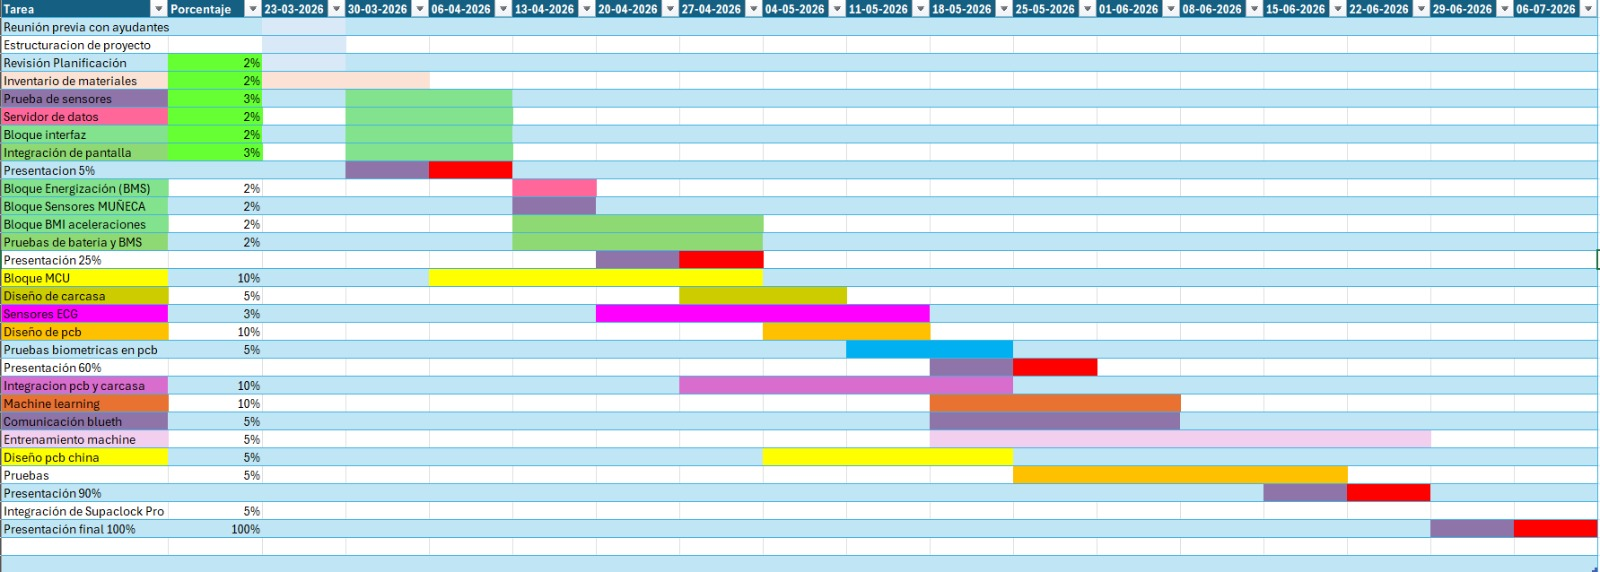
\includegraphics[width=0.95\linewidth, height=0.85\textheight, keepaspectratio]{CartaGantt_actualizada.jpeg}
    \end{center}
\end{frame}

\begin{frame}{Próximos Pasos (Validación de 25\%)}
    \begin{block}{Finalizar Validación de Componentes}
        El objetivo principal de la siguiente etapa es finalizar la validación de componentes, así como comenzar con la de algoritmo de detección de pasos.
    \end{block}
    \vspace{0.3cm}
    \textbf{Objetivos a Corto Plazo:}
    \begin{enumerate}
        \item \textbf{Ensamblaje Power-Up:} Integrar el bloque de energía (LDO+BMS).
        \item \textbf{Integración de Sensores:} Conectar y configurar el resto de sensores (Acelerómetro, ECG, HR + SpO2, batería).
        \item \textbf{Pruebas de Adquisición de Datos:} Se busca guardar datos de los sensores.
        \item \textbf{Algoritmos:} Validar el funcionamiento del contador de pasos.
    \end{enumerate}
\end{frame}

\begin{frame}[focus]
  \Huge Demostración Técnica Preliminar
\end{frame}

\begin{frame}[allowframebreaks]{Referencias Bibliográficas}
    \begin{thebibliography}{9}
        \bibitem{Kushlev2016}
        K. Kushlev, J. Proulx, and E. W. Dunn, ``Silence your phones: Smartphone notifications increase inattention and hyperactivity symptoms,'' \textit{Proceedings of the 2016 CHI Conference on Human Factors in Computing Systems}, 2016, pp. 1011--1020.
        
        \bibitem{Pielot2014}
        M. Pielot, K. Church, and R. de Oliveira, ``An in-situ study of mobile phone notifications,'' \textit{16th International Conference on Human-Computer Interaction with Mobile Devices \& Services}, 2014, pp. 233--242.
        
        \bibitem{Shin2019}
        G. Shin, MC. Jarrahi, Y. Fei, and A. Karami, ``Wearable activity trackers, accuracy, adoption, acceptance and health impact,'' \textit{Biomedical engineering letters}, vol. 9, no. 1, pp. 45-52, 2019. (Previene la inactividad continua y combate silenciosamente el sedentarismo y la obesidad).
    \end{thebibliography}
\end{frame}

\end{document}
